
\begin{figure}[ht]
	\centerline{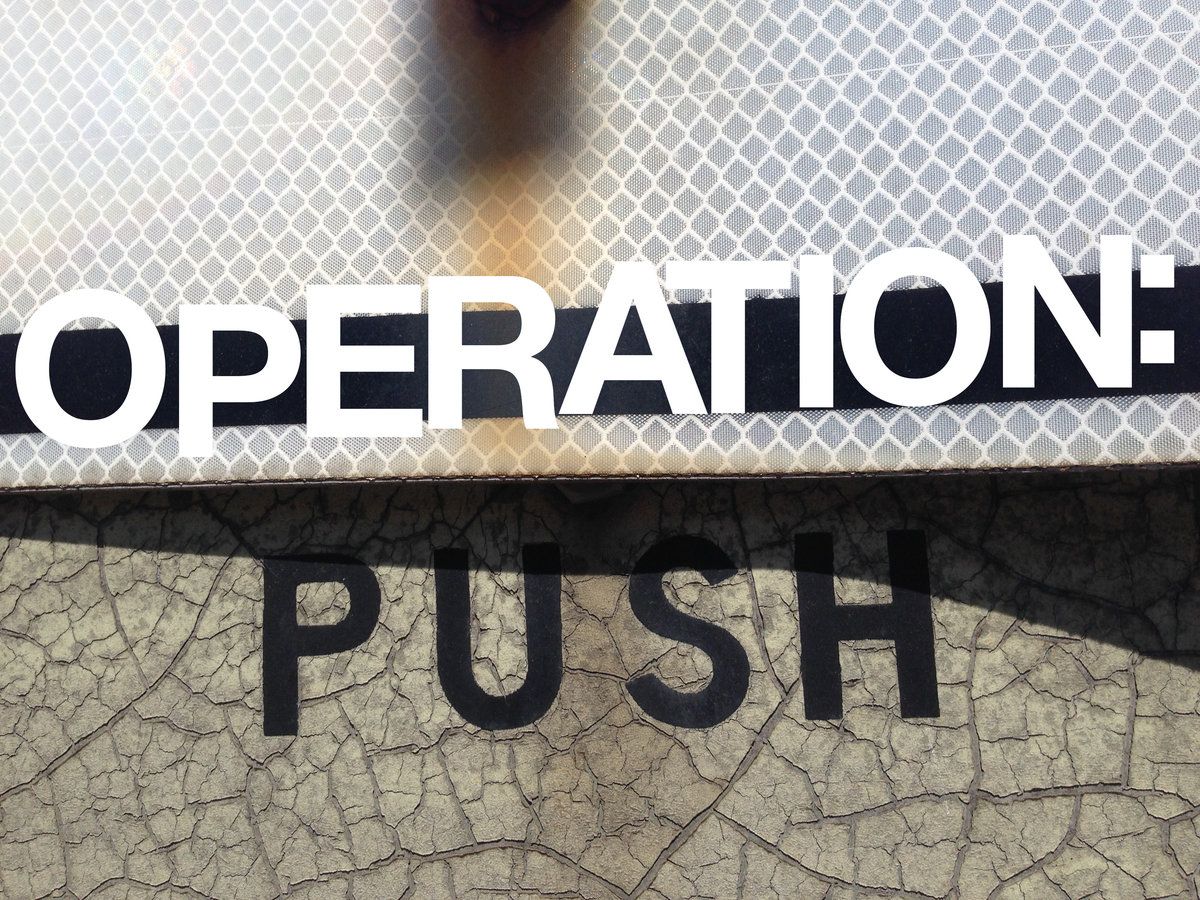
\includegraphics[width=0.60\textwidth]{Figures/dapgit3.jpg}}
	\caption{Push Operation}
	\label{Push Operation}
\end{figure}

\section {Pengertian }
\subsection {Push Operation}
Bekerja dalam satu proyek secara bersama-sama sudah menjadi hal yang lumrah sekarang ini. Termasuk juga proyek-proyek dalam dunia komputer yang sebagian besar menuliskan kode untuk menciptakan software, sistem informasi, aplikasi, atau apa pun namanya. Salah satu sistem yang banyak dipakai untuk membantu pengerjaan proyek bersama tersebut adalah Source Control Management (SCM) atau disebut juga dengan Version Control System (VCS). Ada banyak contoh produk-produk yang tergolong ke dalam jenis VCS, salah satunya adalah Git. Git adalah VCS yang dibangun oleh Linus Torvalds, dikenal juga sebagai pencipta sistem operasi linux, untuk membantu pengembangan kernel linux. Sebelum menggunakan git, pengembangan kernel linux menggunakan produk VCS bernama BitKeeper. Ketika BitKeeper telah menjadi software yang berbayar dan tidak menjadi produk opensource lagi, maka Linus menciptakan Git sebagai pengganti dalam pengembangan kernel linux. \par
Git adalah VCS yang banyak digunakan saat ini. Banyak pengerjaan proyek bersama menggunakan bantuan Git untuk mengelola artefak proyek. Github, salah satu layanan VCS berbasis Git dengan web-based interface, telah menjadi tempat dikembangkannya proyek-proyek open source diseluruh dunia. Tidak hanya untuk proyek opensource, Github juga dapat digunakan untuk mengerjakan proyek non-opensource. \par
\noindent 
Jadi kenapa Git begitu spesial? \par
\noindent 
Bersifat tersebar, sifat tersebar menyebabkan Git terhindar dari permasalahan kegagalan disatu titik. Jika terjadi kerusakan repo pada salah satu mesin maka dapat dipulihkan dengan menyalin repo yang sama dari mesin yang berbeda. Sifat tersebar juga memudahkan developer untuk menjalankan aplikasi dalam rangka \textit{debugging $  $}karena seluruh artifak proyek ada pada mesin developer tersebut. \par
\noindent 
Opensource, Git dikembangkan dengan tujuan untuk membantu pengembangan kernel linux yang bersifat opensource. Konsep Git dapat dipastikan memenuhi aspek-aspek pendukung pengerjaan proyek-proyek opensource. Satu hal yang pasti bahwa git bebas digunakan tanpa pusing memikirkan lisensi. \par
\noindent 
Snapshots, Bukan Perbedaan, Berbeda $  $dengan VCS lain yang umumnya melakukan pencatatan artefak proyek dengan konsep daftar perubahan file (\textit{list of file-based changes}), $  $ $  $Git melakukan pencatatan terhadap artefak proyek dengan konsep seperti pengambilan foto \textit{(snapshot). $  $}Konsep daftar perubahan file akan menyalin seluruh file pada versi sebelumnya untuk dimasukan pada versi sekarang walaupun tidak terjadi perubahan pada file tersebut. Konsep \textit{snapshot $  $}akan mengambil gambaran artefak proyek secara keseluruhan pada versi pertama. Versi selanjutnya dibuat dengan cara menyimpan perbedaan antara versi sekarang dengan versi selanjutnya ditambah dengan penghubung (\textit{pointer, link}) ke snapshot pada versi sekarang. Jadi konsep snapshot tidak mencatat file yang tidak berubah secara berulang-ulang dan juga tidak kehilangan informasi mengenai versi sebelumnya. \par
\noindent 
Hampir Seluruh Operasi Tidak Melibatkan Jaringan, Konsep terdistribusi pada Git menyebabkan git dapat beroperasi tanpa melibatkan mesin lain secara umum. Hal ini berbeda dengan Centralized VCS(CVCS)yang hampir seluruh operasinya memerlukan koneksi jaringan. Sebagai contoh ketika kita berada di pesawat terbang , kereta api, ataupun area lain yang tidak memiliki jaringan ke server proyek yang sedang dikerjakan, maka kita tidak bisa bekerja secara optimal jika menggunakan CVCS. \par
\noindent 
Git Memiliki Integritas, Segala sesuatu pada Git akan diberi tanda khusus \textit{(checksum) $  $}sebelum disimpan ke dalam database. Hal ini menghindari terjadi\textit{ file corruption} tanpa diketahui oleh Git. Git menggunakan algoritma SHA-1 untuk melakukan \textit{checksum} tersebut. \par
\noindent 
Konsep Tiga Status, $  $Git memiliki 3 status utama dalam melakukan pencatatan terhadap artefak proyek. Konsep 3 status ini adalah kunci utama dalam memahami penggunaan Git secara baik dan benar. Jadi pastikan developer paham dengan konsep 3 status pada Git sebelum menggunakannya. Jika dirasa perlu maka dapat dikumpulkan informasi yang lebih banyak tentang konsep ini untuk mempermudah penggunaan Git kedepannya. File pada Git memiliki salah satu dari 3 status berikut: \textit{commited, modified,} dan \textit{staged. Commited $  $}artinya perubahan terhadap file telah disimpan ke dalam database Git. \textit{Modified} artinya telah terjadi perubahan pada file dan perubahan sama sekali belum disimpan oleh Git. \textit{Staged} artinya perubahan pada file telah tersimpan ke dalam penyimpanan sementara dan siap untuk disimpan ke dalam database. Konsep 3 status menyebabkan proyek pada Git terbagi atas 3 bagian utama yaitu: database Git (\textit{Git directory or Git database or Git Repository}), area kerja (\textit{working directory}), dan area perantara (\textit{staging area})  \par
\noindent 
Database git adalah tempat dimana Git menyimpan seluruh informasi tambahan dan perubahan-perubahan untuk setiap versi artefak proyek. Ini adalah bagian yang sangat penting dari Git dan bagian ini adalah bagian yang akan disalin dalam proses \textit{cloning repository $  $}dari satu mesin ke mesin yang lain. Area kerja adalah folder induk yang mengandung seluruh artefak proyek (file-file) yang sedang dikerjakan. Area perantara adalah tempat menyimpan informasi perubahan terhadap artefak proyek yang siap untuk disimpan ke dalam database Git. Bentuk nyatanya adalah sebuah file yang terletak di dalam direktori Git. Area perantara terkadang disebut juga sebagai index.\vspace{\baselineskip}
\section{Alur kerja Git yang paling umum adalah sebagai berikut} \par


\begin{enumerate}


\item Developer melakukan perubahan terhadap file yang berada pada area kerja \par
\item Developer menyimpan perubahan ke dalam area perantara untuk proses pengambil \textit{snapshot} \par
\item Developer menyimpan perubahan secara permanen ke dalam database Git \par
\vspace{12pt}
\vspace{12pt}
\noindent 
\end {enumerate}


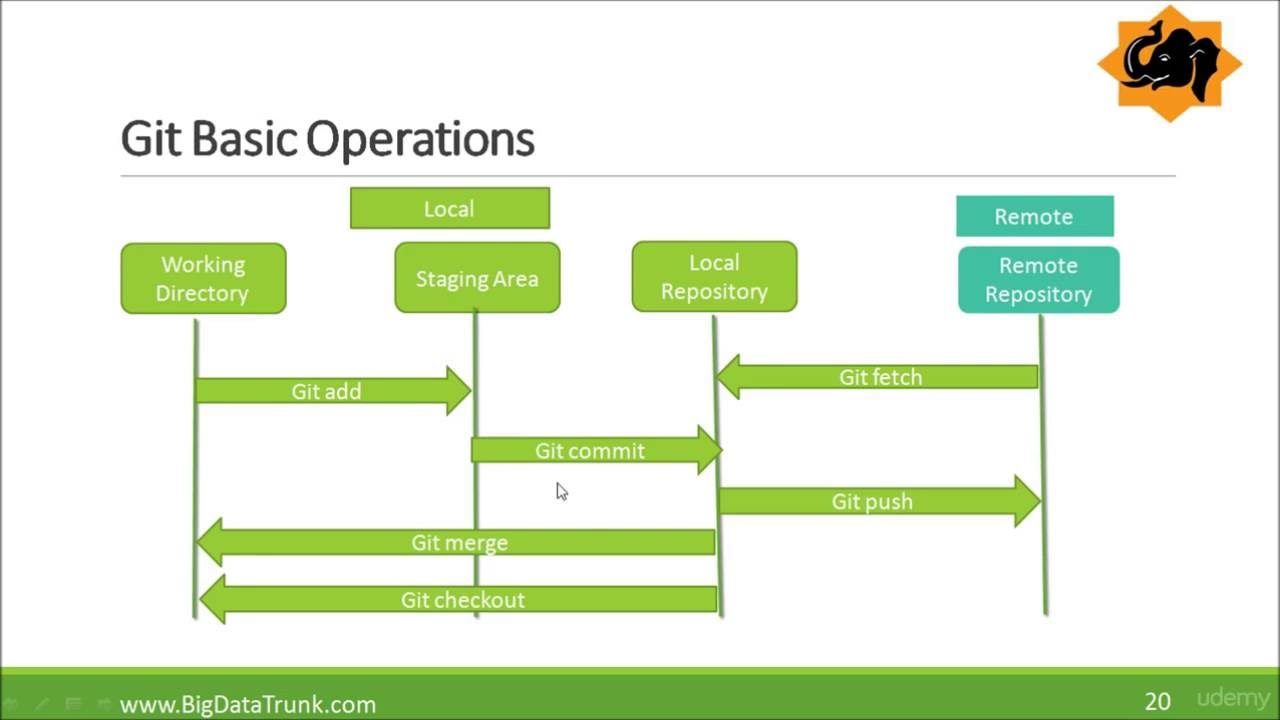
\includegraphics[width=10cm,height=7cm]{Figures/dapgit4.jpg}
\begin{equation}Alur Git \end{equation}

\subsection{Pengertian Lanjutan}

Mungkin sudah terlalu sering kita bekerja mandiri pada project pribadi, disini saya akan menunjukkan bagaimana caranya berkontribusi di project lain. Hal termudah untuk mencapai itu kita cari proyek open sources, apa itu proyek opensources, Proyek perangkat lunak open source merupakan proyek yang memberikan kode program kepada penggunanya secara bebas, dan tak jarang pengembangannya dilakukan secara terbuka: siapapun boleh berkontribusi dalam menulis kode tersebut. Menggunakan perangkat lunak open source tentunya sangat baik, karena selain tidak melakukan pembajakan, kita juga mendukung para pengembang dari perangkat lunak yang kita gunakan. Tetapi, akan lebih baik lagi jika kita juga ikut berkontribusi, mulai dari kontribusi pengunaan, pelaporan bug, sampai dengan kontribusi kode. Kontribusi pada proyek open source akan membantu kita untuk meningkatkan kemampuan pengembangan perangkat lunak.". \par
\vspace{12pt}
\vspace{12pt}
\noindent 
\section{Welcome Contributors} \par
Fork it! \par
Create your feature branch: git checkout -b my-new-feature \par
Commit your changes: git commit -am 'Add some feature' \par
Push to the branch: git push origin my-new-feature \par
Submit a pull request ;) \par
\noindent 
Tahapan berkontribusi yang baik, \par
\noindent 
Cari proyek opensources. \textit{(disini saya sebagai pengembang android saya akan memberikan contoh cara berkontribusi di salah satu proyek opensources pada library android)} \par
\noindent 
\section{Material Tabs} \par
\noindent 
Coba cari cari info tentang aturan kontribusi atau bisa dengan cara melakukan pendekatan pada developer terkait baik via email atau sosial akun. \par
\noindent 
Jika memang telah melakukan pendekatan atau tidak ada jalur lain untuk menempuh jalan tersebut, anda bisa langsung saja untuk melakukan fork project yang akan berkontribusi di dalamnya dimana nantinya kode akan di review oleh pemilik repository untuk di gabungkan atau tidaknya. \par
\noindent 
Setelah selesai fork, maka repository akan masuk ke list repo milik anda, untuk selanjutnya mungkin langsung saja, kali ini masuk pada git command apa aja yang bisa kita gunakan untuk berkontribusi di proyek opensources beserta simulasi yang akan saya contoh kan untuk berkontribusi pada proyek library android - material tabs . \par
\vspace{12pt}
\noindent 
git --help to see another commands cloning project yang suda anda fork ke akun anda \par
\vspace{12pt}
\noindent 
it clone git@github.com:CreatorB/MaterialTabs.git \par
\noindent 
untuk memudahkan development, hendaknya kita menambahkan repository pusat dengan lokal milik kita agar tidak terjadi konflik dengan kontributor lainnya. git remote add <nama-repo> <alamat-repo> \par
\noindent 
git remote add upstream git://github.com/neokree/MaterialTabs.git \par
\noindent 
Setelah remote repositori selesai dan seperti yang saya katakan tadi agar kita tidak hanya asal berkontribusi tapi memang benar benar clear dalam membantu development maka kita hendaknya juga membuat branch baru terlebih dahulu agar tidak merusak history dan nantinya juga akan memudahkan untuk racking code. git checkout -b <nama-cabang> \par
\noindent 
git checkout -b sample-project \par
\noindent 
Okkay sekarang setelah remote dan cabang / branch dibuat maka di cabang baru ini lah kita akan untuk melakukan perubahan kode yang nantinya bisa kita push ke repo pusat. Untuk berpindah branch bisa kita gunakan . git checkout <nama-cabang> dimana di repo lokal saya sekarang ada dua cabang cabang pertama adalah master dan cabang kedua adalah sample-project dan di sample-project saya bisa melakukan banyak perubahan kode. Jika memang ada penambahan file bisa menggunakan git add <nama-file-baru> atau kalo memang banyak file yang ditambahkan dan males add satu per satu, anda bisa langsung menuju root dari repository lalu git add . ya dot / titik berarti menambahkan semua perubahan yang ada di direktori tersebut secara rekursif. Setalah selesai perubahan silahkan lakukan commit, berisi pesan apa yang telah anda kontribusikan / lakukan perubahan. \par
\noindent 
git commit -m "fixing sample project and compile gradle added" \par
\noindent 
Setelah selesai melakukan commit, kita lakukan persiapan untuk pull ke repo pusat, sebelum itu kita pindah branch dulu ke master. \par
\noindent 
git checkout master \par
\noindent 
Setelah itu, kita akan mengambil kode lagi dari pusat, untuk memastikan tidak terdapat konflik pada kontribusi kode kita. Konflik dapat terjadi jika dua atau lebih kontributor melakukan perubahan pada satu berkas, terutama jika perubahan dilakukan pada baris yang sama, terlepas dari apakah tujuan perubahan sama atau tidak. Perintah yang digunakan adalah git fetch dan git merge pada cabang utama. \par
\noindent 
git fetch upstream \par
\noindent 
Setelah fetching selesai, sekarang kita merge dengan master. \par
\noindent 
git merge upstream/master \par
\noindent 
Dengan beberapa proses diatas, setidaknya kita telah bisa memastikan bahwanya tidak ada konflik dengan repo pusat. Sekarang kita kembali ke branch lokal development saya . sample-project \par
\noindent 
git checkout sample-project \par
\noindent 
dan menggabungkan cabang tersebut dengan cabang utama, sehingga kontribusi dapat dikirimkan kembali ke repositori pusat milik neokree, Material Tabs android library, dengan perintah git rebase <nama-branch> \par
\noindent 
git rebase master \par
\noindent 
Sebelum push ke repositori pusat milik neokree, maka terlebih dahulu akan saya push ke repository milik saya hasil fork di awal pembahasan tadi, dimana banyak perubahan yang dilakukan di branch tersebut. \par
\noindent 
git push origin sample-project \par
\noindent 
Setelah di push maka sekarang kita pergi menuju browser untuk melakukan pull request, cek / compare perubahan apa yang telah anda lakukan di branch anda pada branch master milik repo pusat, dan anda juga bisa menyisipkan pesan untuk memberitahukan developer pemilik repo pusat tentang apa yang anda lakukan, setelah yakin terhadap perubahan yang telah anda lakukan silahkan pilih create pull request dan selamat menunggu pemilik repo pusat untuk menanggapi di terima tidaknya kontribusi anda. \par
\vspace{12pt}
\noindent 
\textbf{Cara Push} \par
\vspace{12pt}
\noindent 
Pada dasarnya Git merupakan source control yang berbasis command line, akan tetapi berbagai macam aplikasi GUI Tools sudah banyak di jumpai agar dapat memudahkan kita dalam proses pengerjaan sebuah project atau mempermudah kita yang tidak terlalu mahir dalam penggunaan syntax-syntax tersebut, salah satunya itu SourceTree ini.\vspace{\baselineskip}
\vspace{\baselineskip}
Langsung saja saya mulai untuk proses yang ingin saya contohkan yaitu cara push, pull, commit project ke github dengan menggunakan aplikasi SourceTree. Lalu apa saja yang perlu dipersiapkan ? Berikut adalah beberapa yang perlu anda persiapkan untuk memulai peroses. \par
\noindent 
1 install aplikasi gitbash \par
\noindent 
Bagi~anda yang belum memiliki aplikasi SourceTree, anda dapat men-download nya pada web resmi yang sudah disediakan oleh pengembang aplikasi SourceTree. Aplikasi ini gratis, benar-banar gratis untuk berbagai macam keperluan komersial atau non-komersial. Anda dapat men-download nya pada  web dari githu \par
\noindent 
2~ Akun Github \par
\noindent 
Pastikan anda sudah memiliki akun Github, jika belum memilikinya anda dapat membuatnya terlebih dahulu dengan melakukan register terlebih dahulu, $  $https://github.com/ $  $atau~lihat tutorial cara mendaftar akun Github  Lalu kemudian anda login pada akun Github nya. \par
\vspace{12pt}
\noindent 
Jika sumua keperluan diatas sudah anda siapkan, sekarang kita mulai masuk pada tutorial, ikuti contoh dan prosesnya seperti dibawah ini : \par
\vspace{12pt}
\noindent 
Pertama yang harus anda lakukan adalah untuk menyimpan data-data project pada Github, terlebih dahulu anda membuat repository. Caranya anda klik tanda $  $\textbf{+} pada bagian kanan-atas lalu pilih "\textbf{New Repository}" Lalu anda buat nama untuk repositorinya, lalu klik "Create Repository"  \par
\vspace{12pt}
\noindent 
Setelah itu buka aplikasi SourceTree, jika sudah terbuka aplikasinya maka tampilannya akan seperti gambar dibawh ini. *Pastikan anda sudah login aplikasi SourceTree nya dengan menggunakan akun Github yang anda sudah buat. \par
\vspace{12pt}
\noindent 
repository yang kita buat caranya adalah klik browse pada gambar \textbf{"bumi"}, maka akan tampil semua repository yang kita sudah pernah buat, lalu pilih salah satu repository. Kemudian pada bagian \textbf{Destination Path : }itu adalah lokasi penyimpanan lokal yang kita ingin tempatkan.\vspace{\baselineskip}
\vspace{\baselineskip}
Harus anda ingat lokasi penyimpanan lokal anda, karena ketika kita akan melakukan pull, push, commit dilakukan pada penyimpanan lokal tersebut. Jiak sudah klik \textbf{Clone}. \par
\noindent 
Melakukan Proses Commit  $  \&  $ Push \par
\vspace{12pt}
\noindent 
Kemudian anda buka folder lokal kalian, lalu pindahkan dan letakkan semua file project kalian folder lokal kalian. Saya berikan contoh meletakkan satu file kedalam folder lokal, lihat seperti contoh gambar dibawah ini. \par
\vspace{12pt}
\noindent 
Kemudian anda buka folder lokal kalian, lalu pindahkan dan letakkan semua file project kalian folder lokal kalian. \par
\vspace{12pt}
\noindent 
Lalu anda simpan file yang sudah dibuat, sekarang kembali ke aplikasi SourceTree ketika ada file baru yang di letakkan pada folder lokal maka akan terdeteksi pada aplikasi SourceTree \par
\vspace{12pt}
\noindent 
Kemudian anda pindahkan file yang tadi sudah dibuat menjadi keatas dengan cara klik button \textbf{"Stage All"} $  $kemudian anda isikan komentar yang anda inginkan. Jika sudah anda lakukan Commit, tunggu beberapa saat hingga proses selesai. \par
\vspace{12pt}
\noindent 
Jika sudah maka pada bagian menu \textbf{Push }diatas terdapat notifikasi angka 1 itu artinya ada satu file yang sudah siap di kirim pada server Github. Lalu anda klik menu \textbf{Push} $  $tersebut sehingga muncul \textit{dialog box }lalu anda klik button \textbf{Push} $  $tunggu beberapa saat hingga proses upload selesai. Jika sudah selesai anda bisa cek pada Github, apakah sudah masuk apa belum. \par
\vspace{12pt}
\noindent 
Sampai disini proses commit dan push sudah selesai dilakukan, Kemudian kita akan mencoba melakukan pull, yakni menarik/mengambil file yang ada pada repository. Terlebih dahulu anda membuat file baru pada Github untuk mencoba menarik/mengambil file yang telah dibuat pada repository ke dalam folder lokal. Caranya adalah dengan menekan tombol menu \textbf{Pull}. Kemudian akan muncul \textit{dialog box} Kemudian klik \textbf{OK.} \par
\vspace{12pt}
\noindent 
Tunggu beberapa saat hingga proses selesai dilakukan, jika proses sudah selesai sekarang cek pada folder lokal anda apakah file yang di tarik tadi sudah masuk atau belum. \par
\vspace{12pt}
\vspace{12pt}
\noindent 
Atau jika cara diatas tidak berhasil anda gunakan maka bisa menggunakan cara berikut ini meggunakan gitbash \par
\vspace{12pt}
\noindent 
Setelah kita mempunya akun GitHub dan mengistall software git maka kita bisa langsung meng upload project kita. \par
\noindent 
Buatlah repository di GitHub dengan mengklik icon repo "Create new repository". \par
\noindent 
Kemudian beri nama repository nya lalu beri deskripsi untuk repository yang kita buat jika perlu, kemudian setting public/private, kalau public berarti bisa di akses oleh semua orang, kemudian centang "initialize this repository with a README" dan tambahkan kategori repository jila perlu. \par
\noindent 
kemudian klik "create repository". \par
\noindent 
Jika repository berhasil dibuat, anda akan di berikan kunci akases berupa HTTP/SSH, ini yang akan kita gunakan untuk remote repository dari software GIT. Misal saya punya kunci HTTP http://github.com/acchoblues/APeK.git \par
\noindent 
\begin{enumerate}
\item Setelah anda berhasil membiat repository sekarang klik kanan pada folder project yang akan di upload. \par
\noindent 
\item Klik kanan pada project klik "Git Bash". \par
\noindent 
\item Kemudian akan muncul command prompt / CMD \par
\noindent 
\item Jika anda baru pertama kali meggunakan software GIT, sebaiknya konfigurasi username dan email dulu. \par
\noindent 
\end {enumerate}
Ketik \par
\noindent 

\begin{verbatim}
Git config --global user.name "username anda"  \par
\noindent 
Git config --global user.email isi $ 
 \_  $dengan $  \_  $email $ 
  \_  $anda@ymail.com  \par
\noindent 
\end{verbatim}
Setelah melakukan konfigurasi username dan email, sekarang kita lakukan inisiasi, ketikan  \par
\noindent 
Git init  \par
\noindent 
Kemudian kita tambahkan semua file yang ada dalam folder project kita, ketikan  \par
\noindent 
Git add *  \par
\noindent 
Kemudian kita buat commit project nya, misal disini saya kasih commit  $ " $versi 1.0.0 $ " $ , ketikan  \par
\noindent 
Git commit –m "versi 1.0.0"  \par
\noindent 
Setelah kita buat commit untuk project nya, sekarang kita remote repository yang kita buat tadi, tentunya kita menggunakan kunci HTTP yang ada pada repository tadi, kalo ane kan tadi contoh nya http://github.com/acchoblues/APeK.git , ketikan \par
\noindent 
Git remote add origin http://github.com/acchoblues/APeK.git  \par
\noindent 
Setelah me-remote repository kita tadi, sekarang kita pull project nya, ketikan  \par
\noindent 
Git pull origin master  \par
\noindent 
Terakhir kita kirim project kita ke repository kita, ketikan  \par
\noindent 
Git push origin master  \par
\noindent 
Biasanya ketika kita ketikan perintah push ini, kita akan diminta username dan password kita dan perlu di perhatikan untuk password nya biasa nya ketika kita mengetikan password maka pada command prompt nya tidak ditampilkan karakter apapun. \par
\noindent 
So jangan khawatir tunggu sampai selesai di upload projectnya. \par
\noindent 
kalau sudah selesai proses uploadnya silahkan refresh repository anda, insya allah jika sesuai dengan instruksi di atas maka project anda sudah terupload disana. \par
\vspace{12pt}
\vspace{12pt}

 
\begin{verbatim}

 $  \$  $ \textbf{git init --bare proyekKhadapi} \par

Initialized empty Git repository in F:/proyekkhadpi/ \par

\end{verbatim}
Perintah di atas akan membuat sebuah \textit{bare repository} yang hanya dipakai untuk melakukan sinkronisasi antara pekerjaan Edi dan Bram nantinya. \par
\vspace{12pt}
\noindent 
Di komputer Edi, berbekal dengan flash disk yang mengandung \textit{bare repository} tersebut, ia akan melakukan men-kloning \textit{repository} tersebut dengan memberikan perintah berikut ini: \par
\noindent 
 $  \$  $ \textbf{cd  $  \sim  $/Desktop} \par
\noindent 
\noindent 
\vspace{12pt}
\noindent 
\vspace{12pt}
\noindent 
Sekarang, di folder\textit{  $  \sim  $/Desktop} akan ada sebuah folder \textit{proyek}\textit{Khadapi} yang merupakan kloningan dari yang ada di flash disk. $  $ $  $ Edi hanya perlu meletakkan kode programnya di folder komputer tersebut, dan bukan di \textit{bare repository} di flash disk. \par
\vspace{12pt}
\noindent 
Bram kemudian meminjam flash disk berisi \textit{bare repository} tersebut, dan memberikan perintah yang sama untuk membuat kloning dari \textit{bare repository} yang ada di flash disk ke desktop-nya. \par
\vspace{12pt}
\noindent 
Kedua developer tersebut kemudian bekerja di komputer masing-masing. $  $ $  $ Sebagai contoh, ini adalah simulasi pekerjaan yang dilakukan oleh Edi di repository miliknya: \par
\noindent 
\begin{verbatim}


{echo 'Menu 1' >> menu.txt} \par
 
{echo 'Isi modul 1' >> modul1.txt} \par

{git add .} \par

{git commit -m 'Membuat modul 1'} \par

\end{verbatim}
Edi membuat dua file dengan nama \textit{menu.txt} dan \textit{modul1.txt}. $  $ $  $ Anggap saja ini adalah kode program  \par
\noindent 
Pada saat yang bersamaan, Bram juga menambahkan file pada repository miliknya: \par
\vspace{12pt}
\noindent 
 $  \$  $ \textbf{echo 'Menu 2' >> menu.txt} \par
\noindent 
 $  \$  $ \textbf{echo 'Isi modul 2' >> modul2.txt} \par
\noindent 
 $  \$  $ \textbf{git add .} \par
\noindent 
 $  \$  $ \textbf{git commit -m 'Membuat modul 2'} \par
\noindent 
\vspace{12pt}
\noindent 
Setelah semuanya selesai, Bram men-\textit{push} perubahan yang dilakukannya ke \textit{upstream} di flash disk. $  $ $  $ Ia memberikan perintah berikut ini: \par
\vspace{12pt}
\noindent 
 $  \$  $ \textbf{git push origin master} \par
\noindent 
\vspace{12pt}
\noindent 
Sekarang, commit dengan pesan ‘Membuat modul 2’ milik Bram sudah dipindahkan ke \textit{upstream }di flash disk. $  $ $  $ Untuk memastikannya, ia berpindah ke folder di flash disk, dan memberikan perintah berikut ini: \par
\vspace{12pt}
\noindent 
 $  \$  $ \textbf{cd F:/proyek}\textbf{Khadapi} \par
\noindent 
 $  \$  $ \textbf{git show-branch} \par
\noindent 
[master] Membuat modul 2 \par
\noindent 
\vspace{12pt}
\noindent 
Tugas Bram sudah selesai, $  $ ia kemudian menyerahkan flash disk yang berisi \textit{bare repository} ke Edi. $  $ $  $ Kebetulan Edi juga telah selesai mengerjakan modul 1, sehingga ia berniat men-\textit{push} perubahannya ke \textit{upstream}. $  $ $  $ Akan tetapi Edi akan memperoleh pesan kesalahan seperti berikut ini: \par
\vspace{12pt}
\noindent 
 $  \$  $ \textbf{git push origin master} \par
\noindent 
To file://F:/proyekKhadapi \par
\noindent 
~!~[reject]~~~~   master -> master (fetch first) \par
\noindent 
error: failed to push some refs to 'file://F:/proyekKhadapi' \par
\noindent 
\vspace{12pt}
\noindent 
Pesan kesalahan ini muncul karena pada saat Edi mengerjakan modul 1, $  $ Bram telah duluan men-\textit{push} kode programnya ke \textit{upstream }di flash disk. $  $ $  $ Agar bisa men-\textit{push} ke \textit{upstream}, Edi perlu terlebih dahulu mengambil perubahan yang dibuat oleh Bram di \textit{upstream} dan men-\textit{merge} perubahan tersebut dengan perubahan miliknya. $  $ $  $ Edi memberikan perintah berikut ini: \par
\vspace{12pt}
\noindent 
 $  \$  $ \textbf{git pull} \par
\noindent 
... \par
\noindent 
Auto-merging menu.txt \par
\noindent 
CONFLICT (add/add): Merge conflict in menu.txt \par
\noindent 
Automatic merge failed; fix conflicts and then commit the result. \par
\noindent 
\vspace{12pt}
\noindent 
\vspace{12pt}
\noindent 
Git biasanya cukup pintar dalam melakukan merging file yang konflik. $  $ $  $ Tapi pada kasus ini, baik Edi dan Bram sama-sama menambah item baru pada baris pertama, sehingga Git tidak tahu mana yang harus dipakai. $  $ $  $ Edi perlu memperbaiki konflik ini dengan mengubah file \textit{menu.txt} secara manual menjadi seperti berikut ini: \par
\vspace{12pt}
\vspace{12pt}
\noindent 
Menu 1 \par
\noindent 
Menu 2 \par
\noindent 
\vspace{12pt}
\noindent 
\vspace{12pt}
\noindent 
Setelah itu, Edi akan men-\textit{commit} perubahan ini dengan memberikan perintah berikut ini: \par
\vspace{12pt}
\noindent 
 $  \$  $ \textbf{git add menu.txt} \par
\noindent 
 $  \$  $ \textbf{git commit -m 'Menyesuaikan dengan perubahan dari Bram'} \par
\noindent 
\vspace{12pt}
\noindent 
Sekarang, Edi akan memiliki 3 file, yaitu \textit{menu.txt}, \textit{modul1.txt} dan \textit{modul2.txt.} $  $ $  $ Ini mewakili hasil akhir yang diharapkan. $  $ $  $ Untuk melihat riwayat perubahan, Edi dapat memberikan perintah berikut ini: \par
\noindent 
 $  \$  $ \textbf{git log} \par
\noindent 
commit 8ce2a6bdc83387c2f81c56d60e06fa0ce62a3df8 \par
\noindent 
Merge: 1bcc42b 841b46d \par
\noindent 
Author: Edi <edi@dev.com> \par
\noindent 
Date:~~ Fri Apr 12 06:19:25 2013 +0700 \par
\noindent 
\vspace{12pt}
\noindent 
~~~ Menyesuaikan dengan perubahan dari Bram \par
\noindent 
\vspace{12pt}
\noindent 
commit 841b46d0dea229f55fd215e9cfadcd58b8aa64c2 \par
\noindent 
Author: Bram <bram@dev.com> \par
\noindent 
Date:~~ Fri Apr 11 05:57:37 2013 +0700 \par
\noindent 
\vspace{12pt}
\noindent 
~~~ Membuat modul 2 \par
\noindent 
\vspace{12pt}
\noindent 
commit 1bcc42b2346b95830bd6b3363425a9c8fa3a92f4 \par
\noindent 
Author: Edi <edi@dev.com> \par
\noindent 
Date:~~ Fri Apr 10 05:56:45 2013 +0700 \par
\noindent 
\vspace{12pt}
\noindent 
~~~ Membuat modul 1 \par
\noindent 
\vspace{12pt}
\noindent 
Saat ini perubahan masih ada di repository lokal milik Edi. $  $ $  $ Untuk memindahkan perubahan ke \textit{upstream} yang ada di flash disk, Edi memberikan perintah berikut ini: \par
\vspace{12pt}
\noindent 
 $  \$  $ \textbf{git push} \par
\noindent 
Oke, Edi kemudian  \par
\noindent 
meninggalkan komputer dan menikmati hidupnya untuk sejenak. \par
\noindent 
Kita kembali lagi ke Bram. $  $ Saat ini Bram hanya memiliki kode program modul 2 dan tidak memiliki kode program modul 1 yang dibuat Edi. Bram juga ingin memperoleh kode program terbaru! $  $ Ia meminjam flash disk yang berisi \textit{bare repository}, mencolokkannya di komputer rumahnya, lalu Bram memberikan perintah berikut ini: \par
\vspace{12pt}
\noindent 
 $  \$  $ \textbf{git pull} \par
\noindent 
... \par
\noindent 
Updating 841b46d..8ce2a6b \par
\noindent 
Fast-forward \par
\noindent 
~menu.txt~   $  \vert  $ 1 + \par
\noindent 
 modul1.txt  $  \vert  $ 1 + \par
\noindent 
 2 files changed, 2 insertions(+) \par
\noindent 
 create mode 100644 modul1.txt \par
\noindent 
\vspace{12pt}
\noindent 
\vspace{12pt}
\noindent 
\vspace{12pt}
\noindent 
Kali ini tidak ada konflik saat melakukan \textit{pull} dari \textit{upstream}. $  $ $  $ Hal ini karena Edi sudah menyelesaikan (atau mengatasi) konflik tersebut sebelumnya. $  $ $  $ Sampai pada tahap ini, isi repository Bram akan sama persis dengan milik Edi (terdiri atas 3 file yaitu \textit{menu.txt}, \textit{modul1.txt} dan \textit{modul2.txt}). \par
\vspace{12pt}
\noindent 
Pada contoh ini, Bram dan Edi memakai \textit{bare repository} yang disimpan di sebuah flash disk sebagai perantara. $  $ $  $ Hal ini bukanlah sesuatu yang efisien terutama bila mereka dipisahkan oleh jarak yang jauh. $  $ $  $ Bila komputer mereka sama-sama terkoneksi ke internet, mereka dapat men-\textit{setup} sebuah server Git sebagai \textit{upstream}. $  $ $  $ Selain mendukung protokol git (\textit{native}), Git juga mendukung protokol lainnya seperti HTTP, HTTPS, SSH, dan SCP. $  $ $  $ Sebuah server Git paling mudah dikonfigurasi bila memakai sistem operasi Linux. $  $ $  $ Bila tidak ingin repot-report men-setup server sendiri, Bram dan Edit dapat layanan dari pihak penyedia server seperti GitHub. \par
\vspace{12pt}

